\documentclass[tikz, 12pt]{standalone}

\usepackage{xcolor}
\definecolor{colora}{RGB}{214,76,71}
\definecolor{colorg}{RGB}{84,175,216}
\definecolor{colort}{RGB}{98,174,17}
\definecolor{colorc}{RGB}{253,205,103}
\definecolor{colorn}{RGB}{ 45,45,45}
\definecolor{colord}{RGB}{ 44,46,255}
\definecolor{colorb}{RGB}{ 14,41,89}
\definecolor{colori}{RGB}{255,44,45}

\usepackage{tikz}
\usetikzlibrary{arrows,shapes,backgrounds,shadows,calc,decorations.pathreplacing}

\tikzstyle{blockA} = [text=white,fill=colora, draw=black, ultra thick, rounded corners, drop shadow]
\tikzstyle{blockC} = [text=white,fill=colorc, draw=black, ultra thick, rounded corners, drop shadow]
\tikzstyle{blockG} = [text=white,fill=colorg, draw=black, ultra thick, rounded corners, drop shadow]
\tikzstyle{blockT} = [text=white,fill=colort, draw=black, ultra thick, rounded corners, drop shadow]
\tikzstyle{blockN} = [text=white,fill=colorn, draw=black, ultra thick, rounded corners, drop shadow]
\tikzstyle{blockd} = [text=white,fill=colord, draw=black, ultra thick, rounded corners, drop shadow]
\tikzstyle{blockb} = [text=white,fill=colorb, draw=black, ultra thick, rounded corners, drop shadow]
\tikzstyle{blocki} = [text=white,fill=colori, draw=black, ultra thick, rounded corners, drop shadow]


\tikzstyle{circleA} = [circle, inner color = colora!20, outer color=colora, draw=black, ultra thick, rounded corners, drop shadow]
\tikzstyle{circleC} = [circle, inner color = colorc!20, outer color=colorc, draw=black, ultra thick, rounded corners, drop shadow]
\tikzstyle{circleG} = [circle, inner color = colorg!20, outer color=colorg, draw=black, ultra thick, rounded corners, drop shadow]
\tikzstyle{circleT} = [circle, inner color = colort!20, outer color=colort, draw=black, ultra thick, rounded corners, drop shadow]
\tikzstyle{circleN} = [circle, inner color = colorn!20, outer color=colorn, draw=black, ultra thick, rounded corners, drop shadow]
\tikzstyle{circled} = [circle, inner color = colord!20, outer color=colord, draw=black, ultra thick, rounded corners, drop shadow]
\tikzstyle{circleb} = [circle, inner color = colorb!20, outer color=colorb, draw=black, ultra thick, rounded corners, drop shadow]
\tikzstyle{circlei} = [circle, inner color = colori!20, outer color=colori, draw=black, ultra thick, rounded corners, drop shadow]

\pgfmathdeclarerandomlist{randomColors}{
  {colora}
  {colorc}
  {colorg}
  {colort}
}

\begin{document}

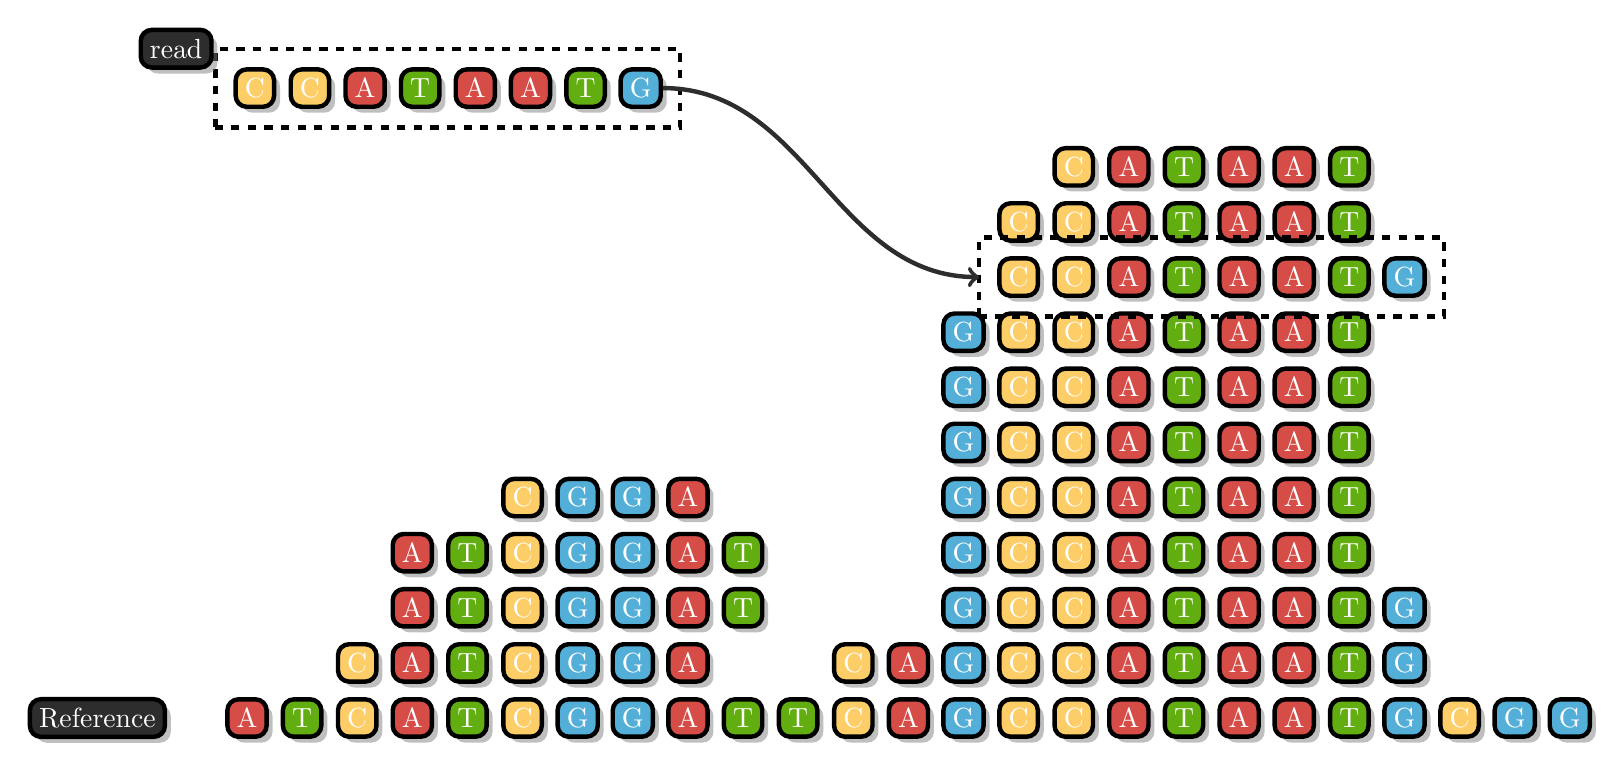
\begin{tikzpicture}

  \node[rectangle,blockA] at  (-2.1,0) {A};
  \node[rectangle,blockT] at  (-1.4,0) {T};
  \node[rectangle,blockC] at  (-0.7,0) {C};
  \node[rectangle,blockC] at  (-0.7,0.7) {C};
  \foreach \x in {0,0.7, ...,2.1}
  \node[rectangle,blockA] at  (0,\x) {A};
  
  \foreach \x in {0,0.7, ...,2.1}
  \node[rectangle,blockT] at  (0.7,\x) {T};

  \foreach \x in {0,0.7, ...,2.8}
  \node[rectangle,blockC] at  (1.4,\x) {C};

  \foreach \x in {0,0.7, ...,2.8}
  \node[rectangle,blockG] at  (2.1,\x) {G};

  \foreach \x in {0,0.7, ...,2.8}
  \node[rectangle,blockG] at  (2.8,\x) {G};

  \foreach \x in {0,0.7, ...,2.8}
  \node[rectangle,blockA] at  (3.5,\x) {A};

  \foreach \x in {0, 1.4, 2.1}
  \node[rectangle,blockT] at  (4.2,\x) {T};

  \foreach \x in {0}
  \node[rectangle,blockT] at  (4.9,\x) {T};

  \foreach \x in {0, 0.7}
  \node[rectangle,blockC] at  (5.6,\x) {C};

  \foreach \x in {0, 0.7}
  \node[rectangle,blockA] at  (6.3,\x) {A};

  \foreach \x in {0, 0.7,...,4.9}
  \node[rectangle,blockG] at  (7,\x) {G};

  \foreach \x in {0, 0.7, ...,6.3}
  \node[rectangle,blockC] at  (7.7,\x) {C};

  \foreach \x in {0, 0.7, ...,7}
  \node[rectangle,blockC] at  (8.4,\x) {C};

  \foreach \x in {0,0.7, ...,7}
  \node[rectangle,blockA] at  (9.1,\x) {A};

  \foreach \x in {0,0.7, ...,7}
  \node[rectangle,blockT] at  (9.8,\x) {T};

  \foreach \x in {0,0.7, ...,7}
  \node[rectangle,blockA] at  (10.5,\x) {A};

  \foreach \x in {0,0.7, ...,7}
  \node[rectangle,blockA] at  (11.2,\x) {A};

  \foreach \x in {0,0.7, ...,7}
  \node[rectangle,blockT] at  (11.9,\x) {T};

  \foreach \x in {0,0.7,1.4,5.6}
  \node[rectangle,blockG] at  (12.6,\x) {G};

  \foreach \x in {0}
  \node[rectangle,blockC] at  (13.3,\x) {C};

  \foreach \x in {14, 14.7}
  \node[rectangle,blockG] at  (\x,0) {G};
  

  %CCATAATG
  \node[rectangle,blockC] at  (-2,8) {C};
  \node[rectangle,blockC] at  (-1.3,8) {C};
  \node[rectangle,blockA] at  (-0.6,8) {A};
  \node[rectangle,blockT] at  (0.1,8) {T};
  \node[rectangle,blockA] at  (0.8,8) {A};
  \node[rectangle,blockA] at  (1.5,8) {A};
  \node[rectangle,blockT] at  (2.2,8) {T};
  \node[rectangle,blockG] (n1) at  (2.9,8) {G};

  \draw[black, dashed, ultra thick] (-2.5,7.5) rectangle (3.4,8.5);
  \draw[black, dashed, ultra thick] (7.2,5.1) rectangle (13.1,6.1);

  \path[->, ultra thick, draw=colorn] (n1) edge [out=0,in=180](7.2,5.6);

  \node[blockN] at (-3,8.5) {read};
  \node[blockN] at (-4,0) {Reference};
\end{tikzpicture}

\end{document}
